\section{Polar coordinates and polar graphs}

\begin{outcome}
\begin{enumerate}
\item[A.]  Understand polar coordinates.

\item[B.]  Convert points between Cartesian and polar coordinates. 
\end{enumerate}
\end{outcome}

You have likely encountered the Cartesian coordinate system in many aspects of mathematics. There is an alternative way to represent points in space, called \textbf{polar
coordinates}\index{polar coordinates}. The idea is suggested in the following picture.

\begin{center}
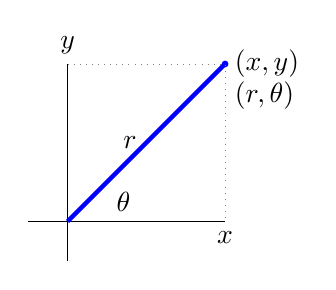
\begin{tikzpicture}
\draw(-0.5,0)--(2,0);
\draw(0,-0.5)--(0,2);
\draw[blue, ultra thick](0,0)--(2,2);
\draw[fill, blue](2,2) circle [radius=1pt];
\draw[help lines, dotted](0,2)--(2,2)--(2,0);
\node[below] at (2,0){$x$};
\node[above] at (0,2){$y$};
\node[above right] at (0.5, 0){$\theta$};
\node[left] at (1,1){$r$};
\node[right] at (2,2){$(x,y)$};
\node[below right] at (2,1.9){$(r, \theta)$};
\end{tikzpicture}
\end{center}

Consider the point above, which would be specified as $(x,y)$ in Cartesian coordinates. We can also specify this point using polar coordinates, which we write as $\tup{r, \theta }$. The number $r$ is the distance from the origin$\tup{0,0}$ to the point, while $\theta $ is the angle shown
between the positive $x$ axis and the line from the origin to the point. In this way, the point can be specified in polar coordinates as $\tup{r, \theta }$.

Now suppose we are given an ordered pair $\tup{r,\theta } $ where 
$r$ and $\theta$ are real numbers. We want to determine the point specified by this ordered pair. We can use $\theta $ to identify a ray
from the origin as follows. Let the ray pass from $\tup{0,0} $
through the point $\tup{\cos \theta ,\sin \theta } $ as shown.

\begin{center}
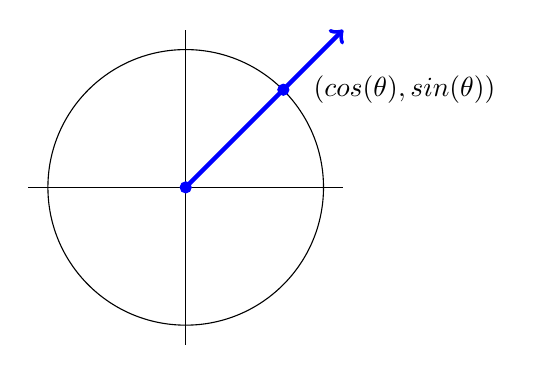
\begin{tikzpicture}
\draw(-2,0)--(2,0);
\draw(0,-2)--(0,2);
\draw(0,0) circle [radius = 1.75];
\draw[->, ultra thick, blue] (0,0)--(2,2);
\draw[fill, blue](0,0) circle [radius=2pt];
\draw[fill, blue](1.24,1.24) circle [radius=2pt];
\node[right] at (1.5, 1.24){$(cos (\theta), sin(\theta))$};
\end{tikzpicture}
\end{center}

The ray is identified on the graph as the line from the origin, through the point $(\cos(\theta),\sin(\theta))$. Now if $r>0,$ go a distance
equal to $r$ in the direction of the displayed arrow starting at $(0,0)$. If 
$r<0,$ move in the opposite direction a distance of $\abs{r}
$. This is the point determined by $\tup{r,\theta }$.

It is common to assume that $\theta $ is in the interval $
[0,2\pi )$ and $r>0.$ In this case, there is a very simple relationship
between the Cartesian and polar coordinates, given by
\begin{equation}
x=r\cos \tup{\theta } ,\ \ y=r\sin \tup{\theta } 
\label{cartpolcoord}
\end{equation}

These equations demonstrate how to find the Cartesian coordinates when we are given the polar coordinates of a point. They can also be used to find the polar coordinates when we know $\tup{x, y }$. A simpler way to do this is the following equations:
\begin{equation}
\begin{array}{l}
r = \sqrt{x^2 + y^2} \\
\\
\tan \tup{\theta} = \frac{y}{x}
\end{array}
\label{polcartcoord}
\end{equation}

In the next example, we look at how to find the Cartesian coordinates of a point specified by polar coordinates. 

\begin{example}{Finding cartesian coordinates}{}
The polar coordinates of a point in the plane are $\tup{5,\pi /6} $.
Find the Cartesian coordinates of this point.
\end{example}

\begin{solution}
The point is specified by the polar coordinates $\tup{5,\pi /6}$. Therefore $r=5$ and $\theta = \pi /6$. 
From \ref{cartpolcoord}
\[
x= r \cos \tup{\theta }= 5\cos \tup{\vspace{0.05in}\frac{\pi }{6}} = \vspace{0.05in}\frac{5}{2}\sqrt{3}
\]
\[
y= r \sin \tup{\theta } = 5\sin \tup{\vspace{0.05in}\frac{\pi }{6}} = \vspace{0.05in}\frac{5}{2}
\]
Thus the Cartesian coordinates are $\tup{\vspace{0.05in}\frac{5}{2}\sqrt{3}, \vspace{0.05in}\frac{5}{2}}$. The point is shown in the below graph. 

\begin{center}
\begin{tikzpicture}[scale=0.5]
\draw(-5,0)--(5,0);
\draw(0,-4)--(0,4);
\draw[help lines, blue, dotted](0, 2.5)--(4.33, 2.5)--(4.33,0);
\draw[fill, blue] (4.33, 2.5) circle [radius=4pt];
\node[right] at (4.33, 2.5){$(\frac{5}{2}\sqrt{3}, \frac{5}{2})$};
\end{tikzpicture}
\end{center}
\end{solution}

Consider the following example of the case where $r < 0$. 

\begin{example}{Finding cartesian coordinates}{}
The polar coordinates of a point in the plane are $\tup{-5,\pi /6} .$
Find the Cartesian coordinates.
\end{example}

\begin{solution}
For the point specified by the polar coordinates $\tup{-5, \pi /6 }$,
$r=-5$, and $x\theta = \pi /6$. 
From \ref{cartpolcoord}
\[
x= r \cos \tup{\theta }= -5\cos \tup{\vspace{0.05in}\frac{\pi }{6}} = -\vspace{0.05in}\frac{5}{2}\sqrt{3}
\]
\[
y= r \sin \tup{\theta } = -5\sin \tup{\vspace{0.05in}\frac{\pi }{6}} = -\vspace{0.05in}\frac{5}{2}
\]
Thus the Cartesian coordinates are $\tup{-\vspace{0.05in}\frac{5}{2}\sqrt{3}, -\vspace{0.05in}\frac{5}{2}}$. The point is shown in the following graph.

\begin{center}
\begin{tikzpicture}[scale=0.5]
\draw(-5,0)--(5,0);
\draw(0,-4)--(0,4);
\draw[help lines, blue, dotted](0, -2.5)--(-4.33, -2.5)--(-4.33,0);
\draw[fill, blue] (-4.33, -2.5) circle [radius=4pt];
\node[left] at (-4.33, -2.5){$(-\frac{5}{2}\sqrt{3}, -\frac{5}{2})$};
\end{tikzpicture}
\end{center}

Recall from the previous example that for the point specified by $\tup{5, \pi /6 }$, the Cartesian coordinates are $\tup{\vspace{0.05in}\frac{5}{2}\sqrt{3}, \vspace{0.05in}\frac{5}{2}}$. Notice that in this example, by multiplying $r$ by $-1$, the resulting Cartesian coordinates are also multiplied by $-1$. 
\end{solution}

The following picture exhibits both points in the above two examples to
emphasize how they are just on opposite sides of $\tup{0,0} $ but at
the same distance from $\tup{0,0} $.

\begin{center}
\begin{tikzpicture}[scale=0.5]
\draw(-5,0)--(5,0);
\draw(0,-4)--(0,4);
\draw[help lines, blue, dotted](0, 2.5)--(4.33, 2.5)--(4.33,0);
\draw[fill, blue] (4.33, 2.5) circle [radius=4pt];
\node[right] at (4.33, 2.5){$(\frac{5}{2}\sqrt{3}, \frac{5}{2})$};
\draw[help lines, blue, dotted](0, -2.5)--(-4.33, -2.5)--(-4.33,0);
\draw[fill, blue] (-4.33, -2.5) circle [radius=4pt];
\node[left] at (-4.33, -2.5){$(-\frac{5}{2}\sqrt{3}, -\frac{5}{2})$};
\draw[blue, ultra thick](-4.33, -2.5)--(4.33, 2.5);
\end{tikzpicture}
\end{center}

In the next two examples, we look at how to convert Cartesian coordinates to polar coordinates. 

\begin{example}{Finding polar coordinates}{}
Suppose the Cartesian coordinates of a point are $\tup{3,4} $. Find
a pair of polar coordinates which correspond to this point.
\end{example}

\begin{solution}
Using equation \ref{polcartcoord}, we can find $r$ and $\theta$. Hence $r=\sqrt{3^{2}+4^{2}}=5$. It remains to identify the angle $\theta$ between the positive $x$ axis and the line from the origin to the point. Since both the $x$ and $y$ values are positive, the point is in the
first quadrant. Therefore, $\theta$ is between $0$ and $\pi /2\ $. 
Using this and \ref{polcartcoord}, we have to solve:
\[
\tan\tup{\theta }=\frac{4}{3}
\]
Conversely, we can use equation \ref{cartpolcoord} as follows:
\[
3=5\cos \tup{\theta } 
\]
\[
4 = 5\sin \tup{\theta } 
\]
Solving these equations, we find that, 
approximately, $\theta =0.\, 927\,295$ radians.
\end{solution}

Consider the following example.

\begin{example}{Finding polar coordinates}{}
Suppose the Cartesian coordinates of a point are $\tup{-\sqrt{3},1}$
. Find the polar coordinates which correspond to this point.
\end{example}

\begin{solution}
Given the point $\tup{-\sqrt{3}, 1}$, 
\begin{eqnarray*}
r &=& \sqrt{ 1^2 + (-\sqrt{3})^2}\\
&=& \sqrt{1 + 3}\\
&=&2
\end{eqnarray*}
 In this case, the point is in the second quadrant since the $x$ value is negative and the $y$ value is positive. Therefore, $\theta$ will be between $\pi/2$ and $\pi$.
Solving the equations
\[
-\sqrt{3}= 2 \cos \tup{\theta}
\]
\[
1 = 2 \sin \tup{\theta} 
\]

we find that $\theta = 5\pi /6.$
Hence the polar coordinates for this point are $\tup{2, 5\pi /6 }$.
\end{solution}

Consider this example. Suppose we used $r=-2$ and $\theta =2\pi -\tup{\pi /6} = 11\pi /6 $. These coordinates specify the same point as above. Observe that there are infinitely many ways to identify this
particular point with polar coordinates. In fact, every point can be represented with polar coordinates in infinitely many ways. Because of this, it will usually be
the case that $\theta $ is confined to lie in some interval
of length $2\pi $ and $r>0$, for real numbers $r$ and $\theta $. 

Just as with Cartesian coordinates, it is possible to use
relations between the polar coordinates to specify points in the plane. The
process of sketching the graphs of these relations is very similar to that used to sketch
graphs of functions in Cartesian coordinates. Consider a relation between polar coordinates of the form, $r=f\tup{\theta }$. To graph such a relation, first make a table of
the form 
\begin{equation*}
\begin{tabular}{|l|l|}
\hline
$\theta $ & $r$ \\ \hline
$\theta _{1}$ & $f\tup{\theta _{1}} $ \\ \hline
$\theta _{2}$ & $f\tup{\theta _{2}} $ \\ \hline
$\vdots $ & $\vdots $ \\ \hline
\end{tabular}
\end{equation*}
Graph the resulting points and connect them with a curve. The
following picture illustrates how to begin this process.

\begin{center}
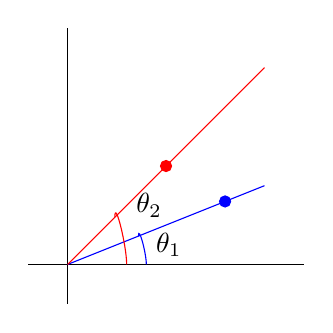
\begin{tikzpicture}
\draw(-0.5,0)--(3,0);
\draw(0,-0.5)--(0,3);
\draw[blue](0,0)--(2.5,1);
\draw[red](0,0)--(2.5,2.5);
\draw[fill,blue] (2,0.8) circle [radius=2pt];
\draw[fill,red] (1.25,1.25) circle [radius=2pt];
\draw[blue](1,0) to [out=90, in=90] (0.9,0.36); 
\draw[red](0.75,0) to [out=90, in=90] (0.6,0.6); 
\node[right] at (1,0.25){$\theta_1$};
\node[right] at (0.75, 0.75){$\theta_2$};
\end{tikzpicture}
\end{center}

To find the point in the plane corresponding to the ordered pair $\tup{f\tup{
\theta } ,\theta } $, we follow the same process as when finding the point corresponding to $\tup{r, \theta }$.

Consider the following example of this procedure, incorporating computer software.

\begin{example}{Graphing a polar equation}{}
Graph the polar equation $r=1+\cos \theta$.
\end{example}

\begin{solution}
We will use the computer software {\em Maple\em} to complete this example. The command which produces the polar graph of the above equation is: $>$ plot(1+cos(t),t=
0..2*Pi,coords=polar). Here we use $t$ to represent the variable $\theta$ for convenience. The command tells Maple that $r$
is given by $1+\cos \tup{t} $ and that $t\in \mat{0,2\pi}$.

\begin{picture}(1,120)
\put(110,-25){
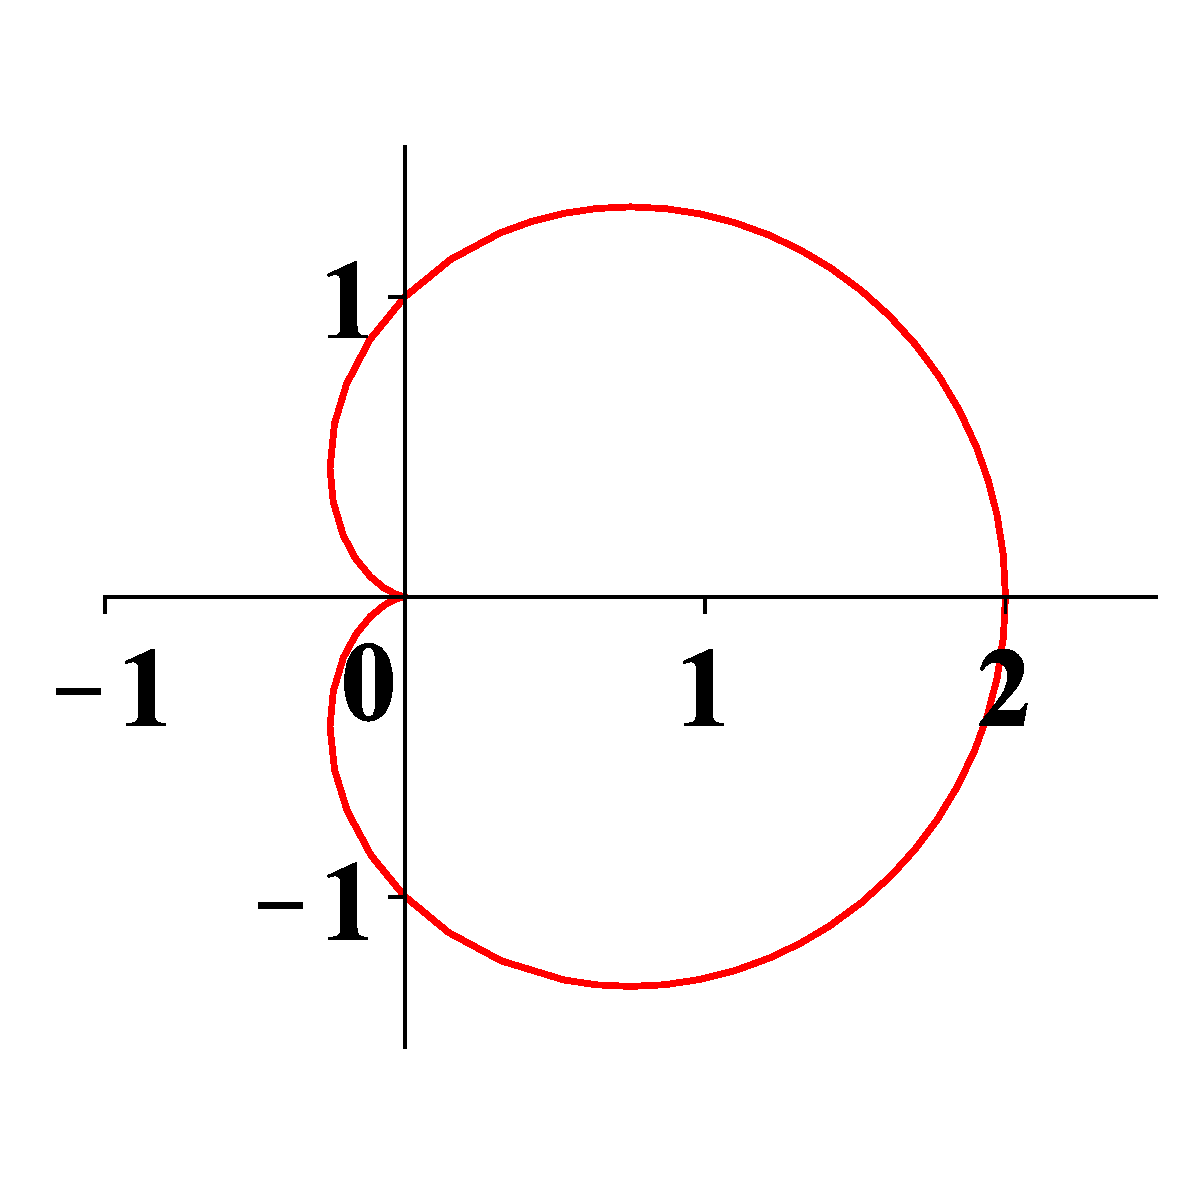
\includegraphics[bb=0 0 400
400,totalheight=3cm]{figures/cardioid.eps}
\put(30,73){\large{x}}
\put(-35,128){\large{y}}}
\end{picture}

The above graph makes sense when considered in terms of trigonometric functions. Suppose $\theta =0,r=2$ and let $\theta $ increase to $\pi /2$. As $\theta$ increases, $\cos \theta $ decreases to 0. Thus the line from the origin to the point on the curve should get shorter as $\theta $ goes from $0$ to $\pi /2$. As $\theta$ goes from $\pi /2$ to $\pi$, $\cos
\theta $ decreases, eventually equalling $-1$ at $\theta =\pi$. Thus $r=0$
at this point. This scenario is depicted in the above graph, which shows a function called a \textbf{cardioid}\index{cardioid}.

The following picture illustrates the
above procedure for obtaining the polar graph of $r=1+\func{cos}(\theta)$. In this picture, the
concentric circles correspond to values of $r$ while the rays from the
origin correspond to the angles which are shown on the picture. The dot on the ray corresponding to the angle $\pi/6$ is located at a distance of $r = 1+\func{cos}(\pi/6)$ from the origin. The dot on the ray corresponding to the angle $\pi/3$
is located at a distance of $r = 1+\func{cos}(\pi/3)$ from the origin and so
forth. The polar graph is obtained by connecting such points with a smooth
curve, with the result being the figure shown above. 

\begin{picture}(1,290)
\put(30,-58){
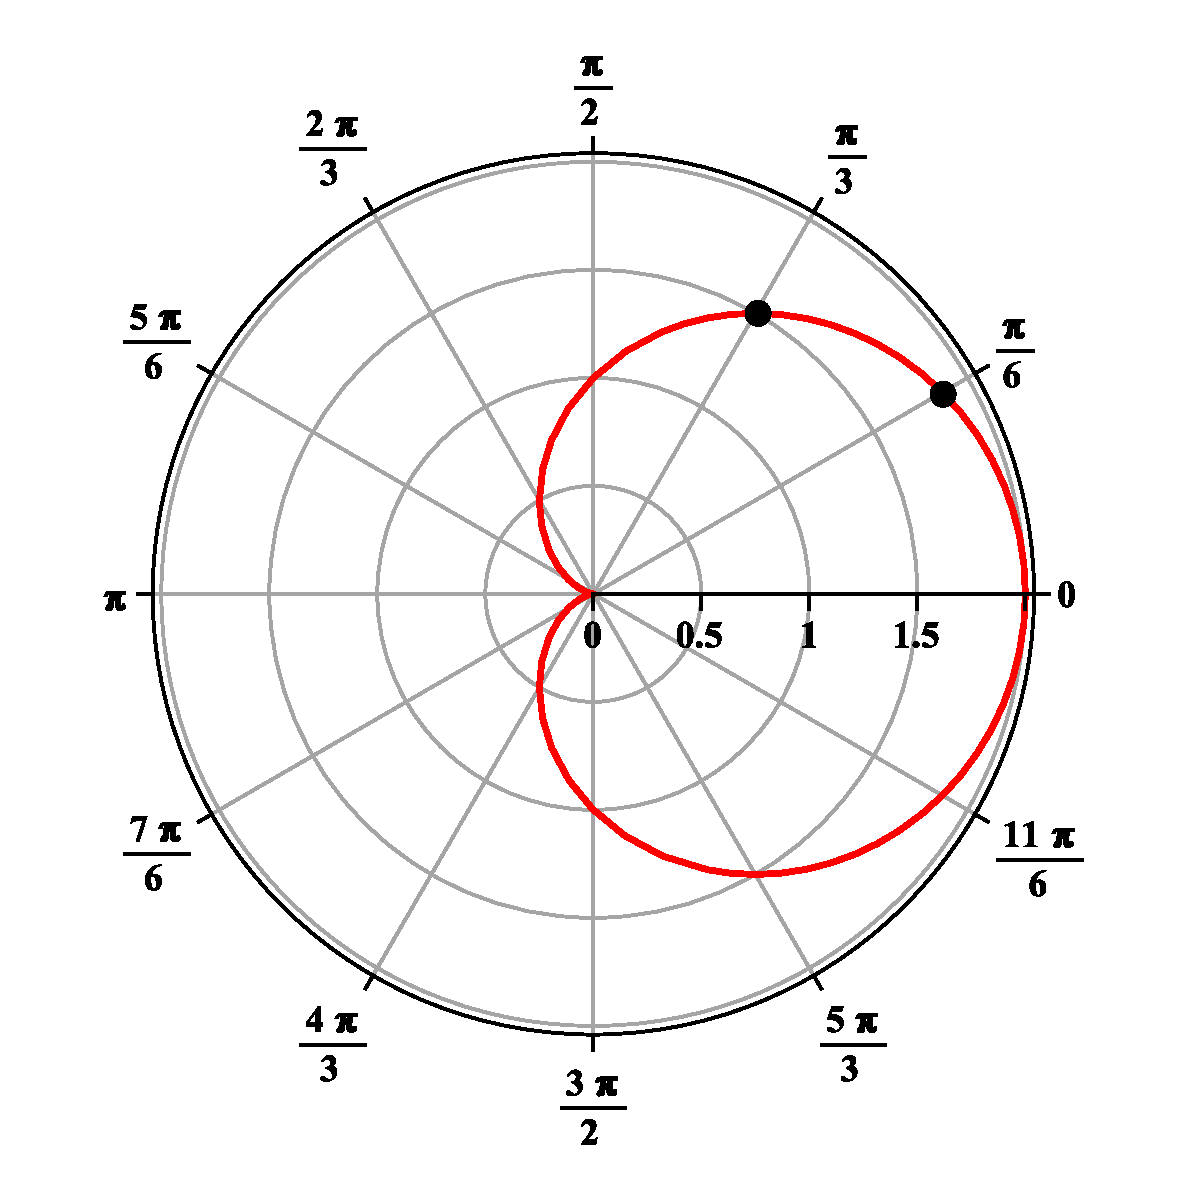
\includegraphics[bb=0 0 400
400,totalheight=7cm]{figures/25aprilcardioid.eps}
%\put(85,128){\large{x}}
%\put(-117,328){\large{y}}\put(80,170){$y=\func{ln}(x)$}
%\put(-90,328){$y=\func{exp}(x)$}
}
\end{picture}
\end{solution}

Consider another example of constructing a polar graph.

\begin{example}{A polar graph}{}
Graph $r=1+2\cos \theta $ for $\theta \in \mat{
0,2\pi}$.
\end{example}

\begin{solution}
The graph of the polar equation $r=1+2\cos \theta $ for $\theta \in \mat{
0,2\pi}$ is given as follows. 

\begin{picture}(1,127)
\put(110,-25){
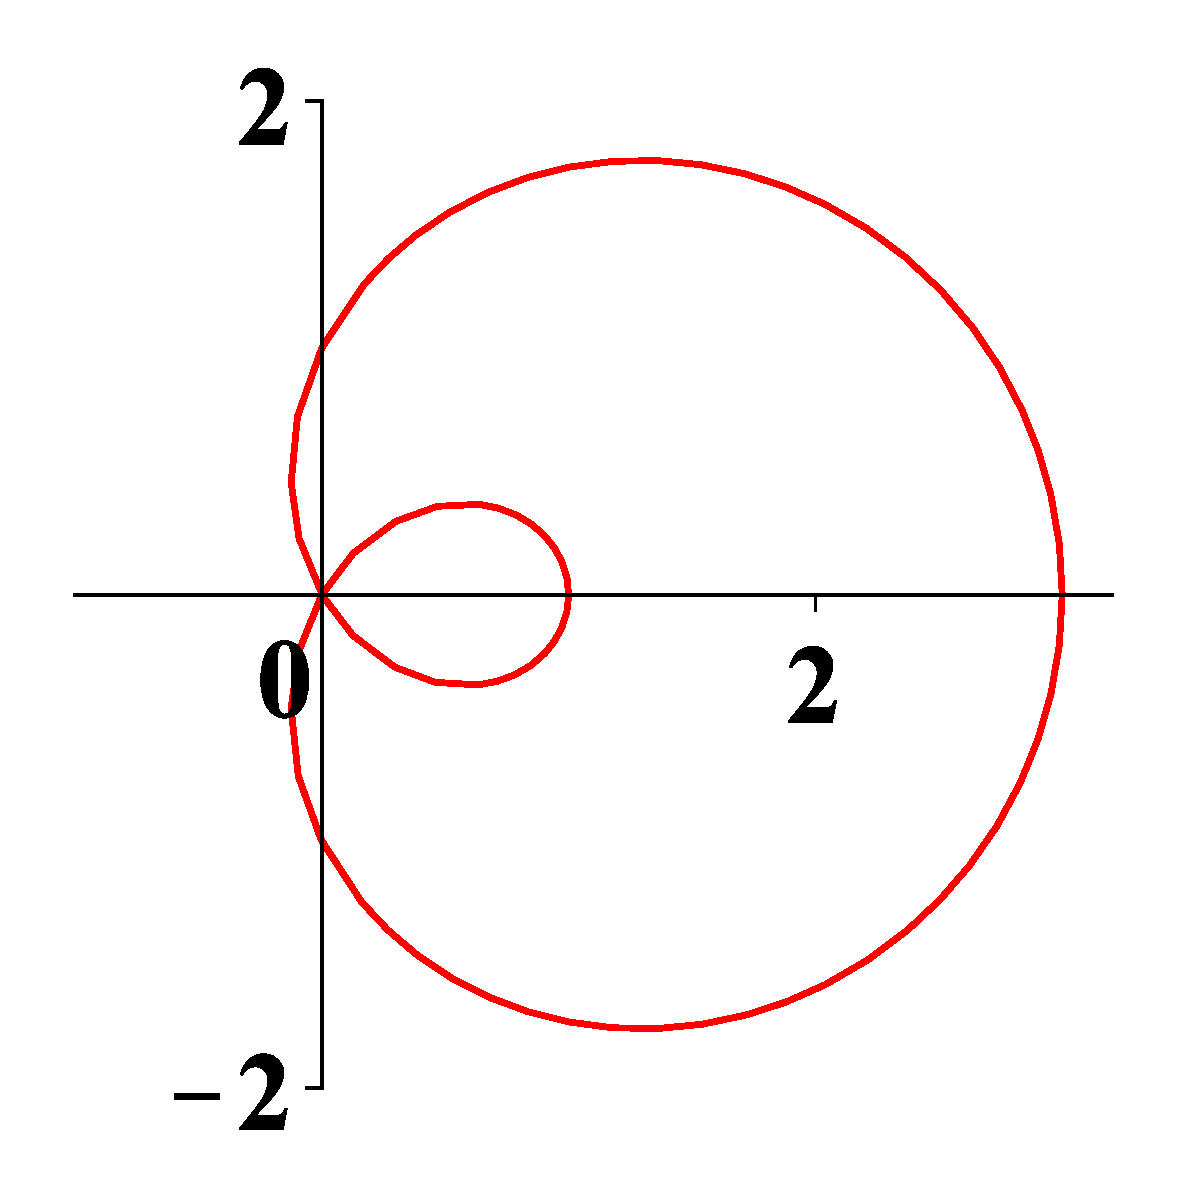
\includegraphics[bb=0 0 400
400,totalheight=3cm]{figures/polarpretty2.eps}
\put(34,79){\large{x}}
\put(-47,138){\large{y}}}
\end{picture}

To see the way this is graphed, consider the following picture. First the
indicated points were graphed and then the curve was drawn to connect the points. When done by a computer, many more points are used to create a more accurate picture.  

Consider first the following table of points. 
\begin{equation*}
\begin{tabular}{|l|l|l|l|l|l|l|l|l|}
\hline
$\theta $ & $\pi /6$ & $\pi /3$ & $\pi /2$ & $5\pi /6$ & $\pi $ & $4\pi /3$
& $7\pi /6$ & $5\pi /3$ \\ \hline
$r$ & $\sqrt{3}+1$ & $2$ & $1$ & $1-\sqrt{3}$ & $-1$ & $0$ & $1-\sqrt{3}$ & $%
2$ \\ \hline
\end{tabular}%
\end{equation*}

Note how some entries in the table have $r<0.$ To graph these points, simply move in the opposite direction. These types of points are responsible for the small loop on the inside of the
larger loop in the graph. 

\begin{picture}(1,290)
\put(30,-58){
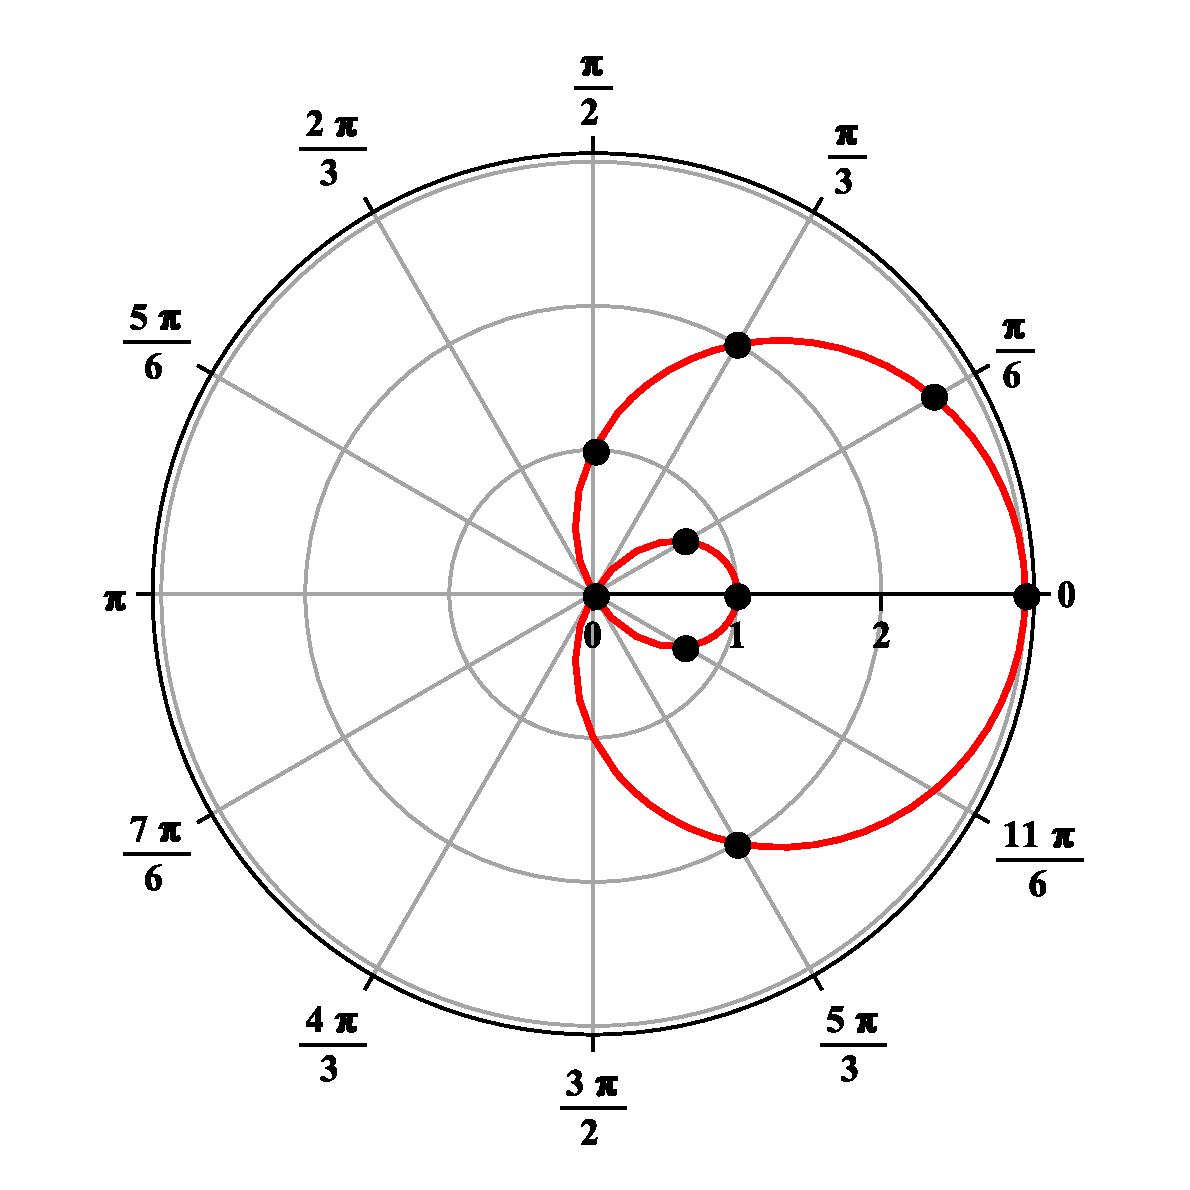
\includegraphics[bb=0 0 400
400,totalheight=7cm]{figures/26aprilwriggly.eps}
%\put(85,128){\large{x}}
%\put(-117,328){\large{y}}\put(80,170){$y=\func{ln}(x)$}
%\put(-90,328){$y=\func{exp}(x)$}
}
\end{picture}
\end{solution}

The process of constructing these graphs can be greatly facilitated by computer software. However, the use of such software should not replace understanding the steps involved.

The next example shows the graph for the equation $r=3+\sin \tup{
\displaystyle
\frac{7\theta }{6}}$. For complicated polar graphs, computer software is used to facilitate the process. 

\begin{example}{A polar graph}{}
Graph $r=3+\sin \tup{\displaystyle \frac{7\theta }{6}%
} $ for $\theta \in \mat{0,14\pi}$.
\end{example}

\begin{solution}

\begin{picture}(1,127)
\put(110,-25){
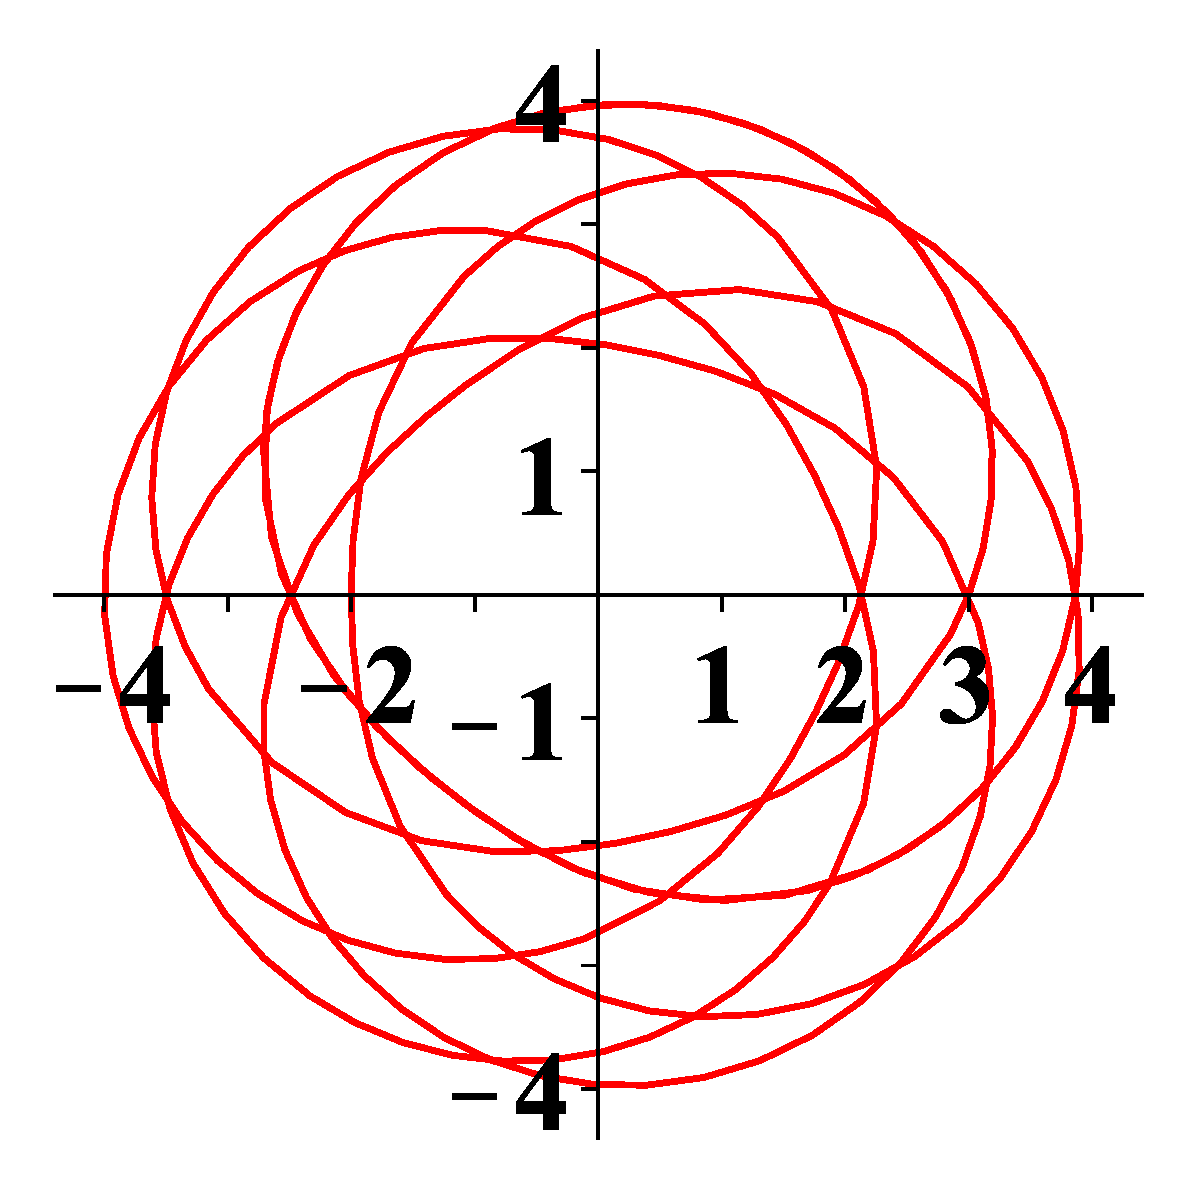
\includegraphics[bb=0 0 400
400,totalheight=3cm]{figures/polarpretty.eps}
\put(34,79){\large{x}}
\put(-20,138){\large{y}}}
\end{picture}
\end{solution}

The next example shows another situation in which $r$ can be negative.

\begin{example}{A polar graph: negative $r$}{}
Graph $r=3\func{sin}(4\theta) $ for $\theta \in \mat{0,2\pi}$.
\end{example}

\begin{solution}

\begin{picture}(1,120)
\put(120,-24){
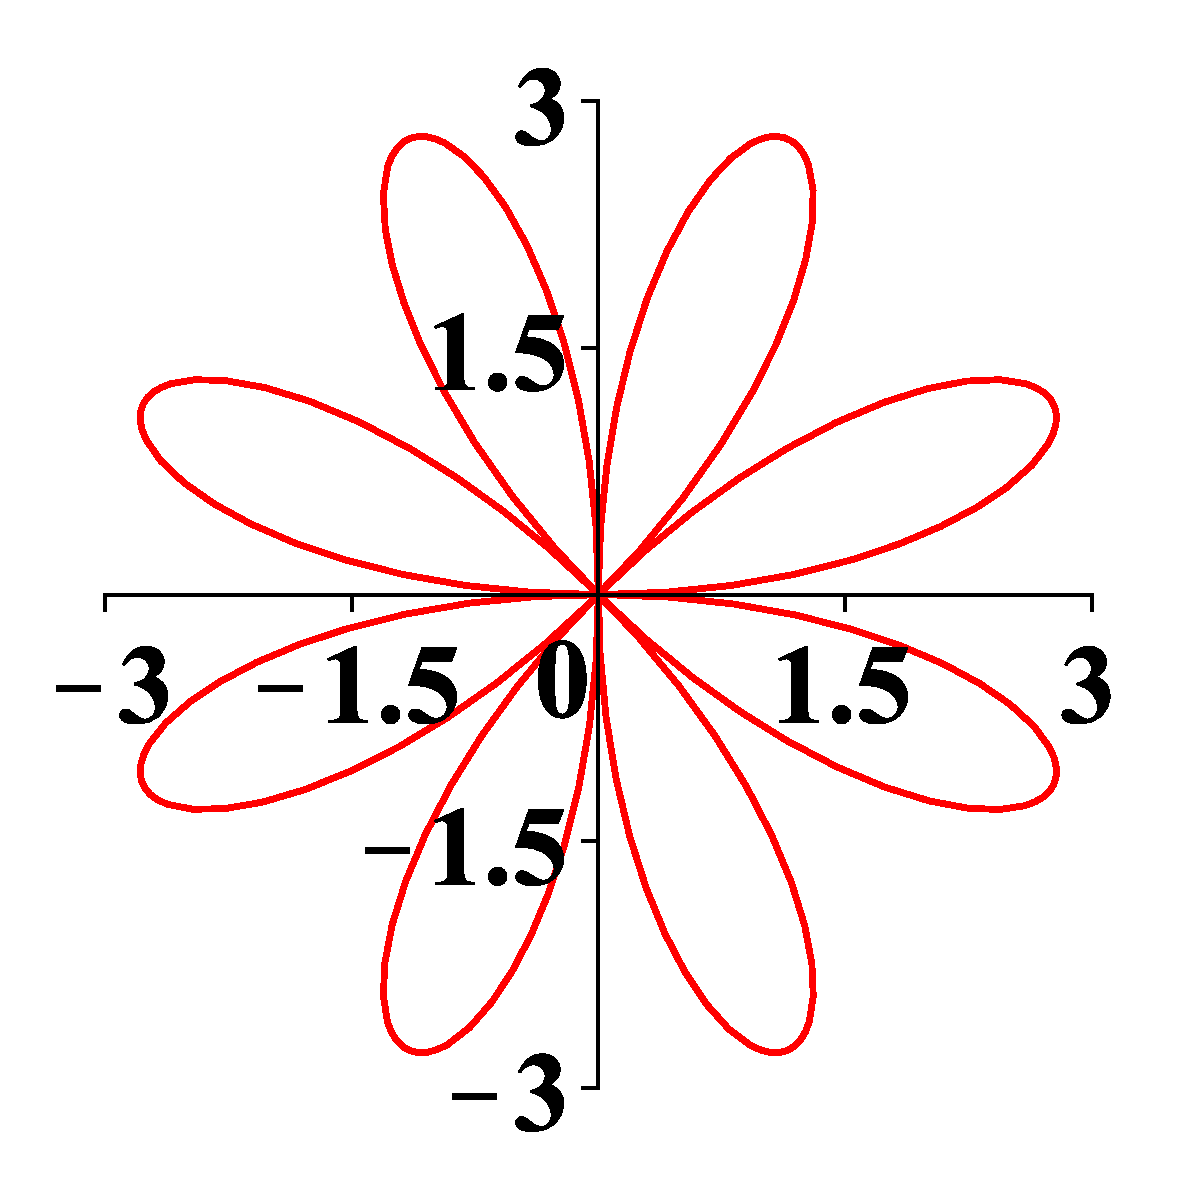
\includegraphics[bb=0 0 400
400,totalheight=3cm]{figures/26aprilrose.eps}}
\put(242,53){\large{x}}
\put(190,105){\large{y}}

\end{picture}
\end{solution}

We conclude this section with an interesting graph of a simple polar equation. 

\begin{example}{The graph of a spiral}{}
Graph $r=\theta$ for $\theta \in [0,2\pi]$.
\end{example}

\begin{solution}
The graph of this polar equation is a spiral. This is the case because as $\theta $ increases, so does $r$.

\begin{picture}(1,290)
\put(30,-58){
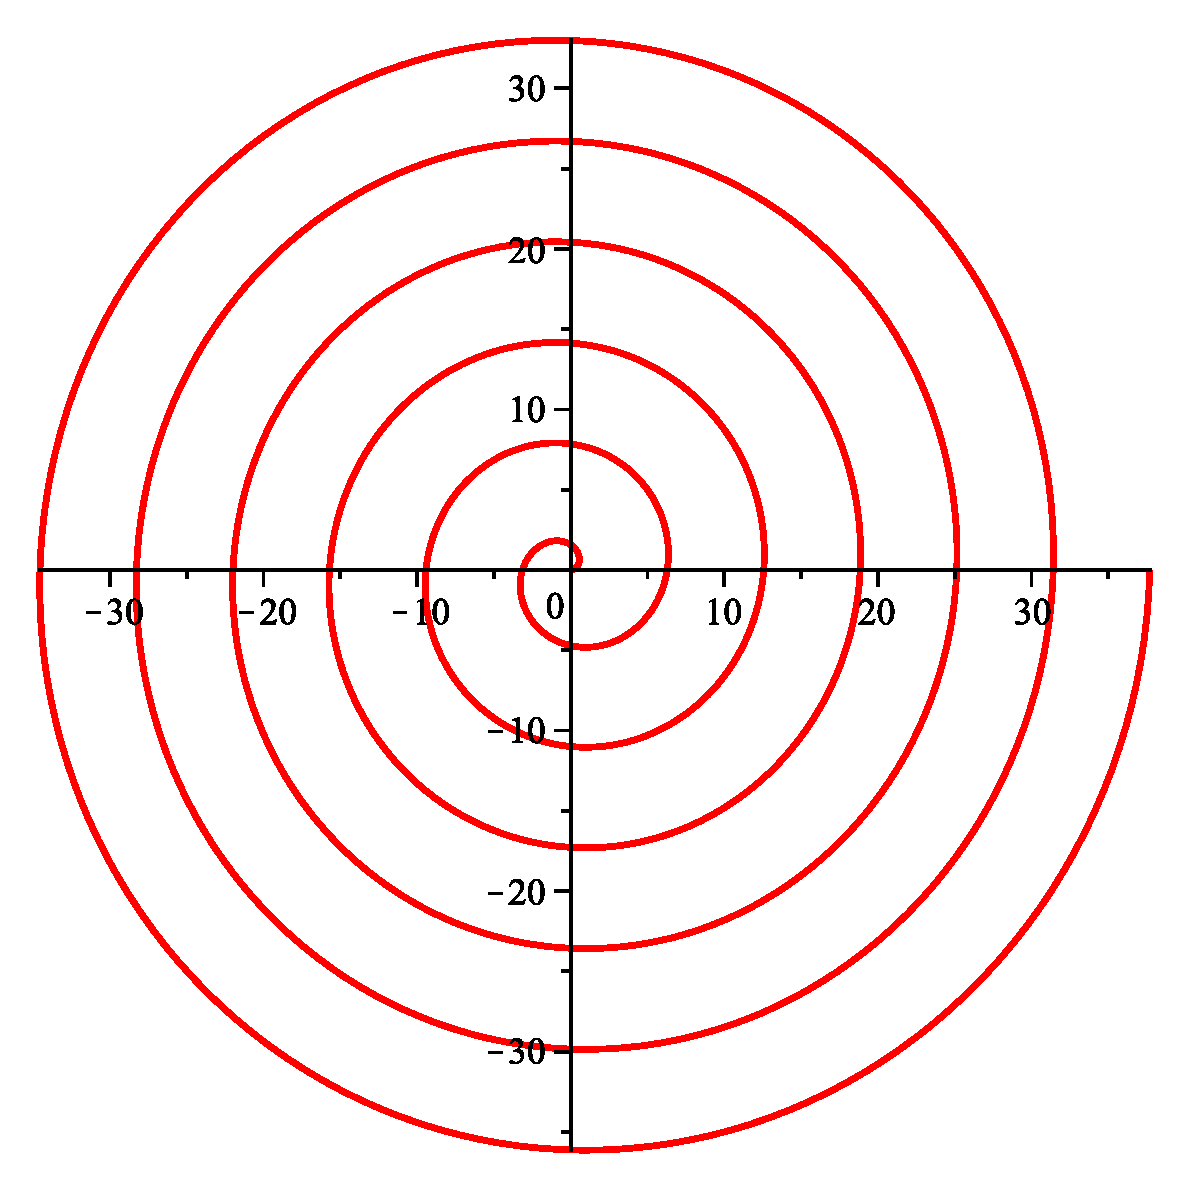
\includegraphics[bb=0 0 400
400,totalheight=7cm]{figures/11mayspiral.eps}
\put(85,205){\large{x}}
\put(-55,335){\large{y}}}
\end{picture}
\end{solution}

In the next section, we will look at two ways of generalizing polar coordinates to three dimensions.
